\chapter{The mower}
\label{ch:mower}

This chapter describes the machine: its dimensions seen from above, how
rolling without slipping ties its motion to the steering angle, where its
blades go in a turn, and how much grass they cut per metre.

\section{The mower seen from above}

\begin{figure}[ht]
  \centering
  \begin{tikzpicture}[scale=4.6, >=Stealth, font=\small]
    % body
    \draw[fill=orange!30, draw=orange!60!black] (-0.45,-0.475)
      rectangle (1.55,0.475);
    % axles
    \draw[very thick, black!60] (0,-0.4) -- (0,0.4);
    \draw[very thick, black!60] (1.2,-0.4) -- (1.2,0.4);
    % wheels
    \foreach \x/\y in {0/0.4, 0/-0.4, 1.2/0.4, 1.2/-0.4}
      \draw[fill=black!80] (\x-0.2,\y-0.075) rectangle (\x+0.2,\y+0.075);
    % deck housing and blade circles
    \draw[fill=black!20, draw=black!60] (0.27,-0.515) rectangle (0.83,0.515);
    \foreach \y in {0.235,-0.235}
      \draw[fill=white, draw=black!70] (0.55,\y) circle (0.25);
    \fill (0.55,0.235) circle (0.012);
    \fill (0.55,-0.235) circle (0.012);
    \draw[->] (0.55,0.235) -- ++(50:0.25) node[pos=0.55, above left=-1pt]
      {$r$};
    % reference point and frame
    \fill (0,0) circle (0.02);
    \node[below left] at (0,0) {$P$};
    \draw[->, thick, blue!70!black] (0,0) -- (0.22,0)
      node[below] {$x$};
    \draw[->, thick, blue!70!black] (0,0) -- (0,0.22) node[left] {$y$};
    % dimensions: wheelbase and deck offset
    \draw[|<->|] (0,-0.66) -- node[below, pos=0.78] {$L$, wheelbase}
      (1.2,-0.66);
    \draw[|<->|] (0,-0.86) -- node[below] {$d$, deck offset} (0.55,-0.86);
    \draw[densely dotted] (0,-0.48) -- (0,-0.9);
    \draw[densely dotted] (1.2,-0.48) -- (1.2,-0.7);
    \draw[densely dotted] (0.55,-0.52) -- (0.55,-0.9);
    % track
    \draw[|<->|] (-0.65,-0.4) -- node[left] {$T$, track} (-0.65,0.4);
    \draw[densely dotted] (-0.2,0.4) -- (-0.69,0.4);
    \draw[densely dotted] (-0.2,-0.4) -- (-0.69,-0.4);
    % cutting width
    \draw[densely dotted] (0.55,0.485) -- (1.85,0.485);
    \draw[densely dotted] (0.55,-0.485) -- (1.85,-0.485);
    \draw[|<->|] (1.8,-0.485) -- node[right] {$w$, cutting width}
      (1.8,0.485);
    \node[orange!50!black] at (1.38,0) {body};
    \node[black!70] at (0.55,0.6) {deck};
  \end{tikzpicture}
  \caption{The mower seen from above, to scale (default dimensions). The
    reference point $P$ is the middle of the rear axle; the mower frame has
    its $x$ axis forward and its $y$ axis to the left. The deck, between the
    axles, holds two blades; each blade tip sweeps a circle of radius $r$,
    and together the two circles cut a band of width $w$.}
  \label{fig:mower}
\end{figure}

\begin{definition}{Mower frame and pose}{pose}
  The \emph{mower frame} has its origin at the middle $P$ of the rear axle,
  its $x$ axis pointing forward and its $y$ axis to the left
  (Figure~\ref{fig:mower}). The \emph{pose} of the mower is
  $q = (x, y, \theta)$: the position of $P$ in the lawn's frame and the
  \emph{heading} $\theta$, the angle from the lawn's $x$ axis to the mower's.
  A point with coordinates $(a, b)$ in the mower frame is, in the lawn's
  frame, at
  \[
    \begin{pmatrix} x \\ y \end{pmatrix}
    + a \begin{pmatrix} \cos\theta \\ \sin\theta \end{pmatrix}
    + b \begin{pmatrix} -\sin\theta \\ \cos\theta \end{pmatrix}.
  \]
\end{definition}

The vectors $u = (\cos\theta, \sin\theta)$ (forward) and
$n = (-\sin\theta, \cos\theta)$ (to the left) are used throughout. The
dimensions are parameters; the default values describe a typical
tractor-style ride-on mower:

\begin{center}
\begin{tabular}{@{}llr@{}}
  \toprule
  symbol & meaning & default \\
  \midrule
  $L$ & wheelbase (rear axle to front axle) & \SI{1.20}{\metre} \\
  $T$ & track (distance between left and right wheels) & \SI{0.80}{\metre} \\
  $\delta_{\max}$ & largest steering angle & \SI{40}{\degree} \\
  $d$ & deck offset (rear axle to the centre of the deck) &
    \SI{0.55}{\metre} \\
  $r$ & radius of the circle swept by a blade tip & \SI{0.25}{\metre} \\
  $y_1, y_2$ & lateral positions of the blade centres &
    $\pm\SI{0.235}{\metre}$ \\
  $w$ & cutting width, $y_1 - y_2 + 2r$ & \SI{0.97}{\metre} \\
  \bottomrule
\end{tabular}
\end{center}

\section{Rolling without slipping}

A wheel that rolls without slipping moves in the direction it points: its
centre has no velocity across the wheel. This single physical assumption,
applied to the rear and front wheels, gives the whole motion model. The real
mower has two front wheels; the model first replaces them by one virtual
wheel in the middle of the front axle (a ``bicycle''), and
Section~\ref{sec:ackermann} comes back to the two real wheels.

\begin{theorem}{Kinematic bicycle model}{bicycle}
  Let $v$ be the signed speed of $P$ (negative in reverse) and $\delta$ the
  steering angle of the virtual front wheel. If no wheel slips sideways, the
  pose evolves as
  \[
    \dot x = v\cos\theta, \qquad
    \dot y = v\sin\theta, \qquad
    \dot\theta = v\,\frac{\tan\delta}{L}.
  \]
  Equivalently, as a function of the signed distance $s$ travelled by $P$,
  the heading turns at the rate
  \[
    \kappa \;=\; \frac{d\theta}{ds} \;=\; \frac{\tan\delta}{L},
  \]
  the \emph{curvature} of the path of $P$.
\end{theorem}

\begin{proof}
  The mower is a rigid body turning at the angular rate $\omega =
  \dot\theta$. The velocity of any of its points $Q$ is therefore
  \[
    v_Q = v_P + \omega\, J(Q - P),
    \qquad J = \begin{pmatrix} 0 & -1 \\ 1 & 0 \end{pmatrix}
  \]
  ($J$ turns a vector by $+90°$; for example $J u = n$ and $J n = -u$).

  \emph{Rear wheels.} Their centres are $P \pm \tfrac T2\,n$, so their
  velocities are $v_P \pm \tfrac T2\,\omega\,J n = v_P \mp \tfrac T2\,\omega
  \,u$. The rear wheels are not steered: they point along $u$, so these
  velocities have no component along $n$. The term $\mp\tfrac T2\,\omega\,u$
  has none either, so $v_P$ has none: $v_P = v\,u$. This is
  $\dot x = v\cos\theta$, $\dot y = v\sin\theta$.

  \emph{Front wheel.} Its centre is $F = P + L\,u$, with velocity
  \[
    v_F = v\,u + \omega L\, J u = v\,u + \omega L\, n .
  \]
  The wheel points along $\cos\delta\,u + \sin\delta\,n$, so $v_F$ must be
  parallel to it: $(v, \omega L) \parallel (\cos\delta, \sin\delta)$, that
  is $\omega L\cos\delta = v\sin\delta$, or $\omega = v\tan\delta / L$.
  Finally $\kappa = d\theta/ds = \dot\theta / v = \tan\delta / L$.
\end{proof}

\begin{inwords}
  The middle of the rear axle always moves straight ahead, like the back of
  a bicycle: its path is tangent to the mower. How fast the path bends
  depends only on the steering angle and the wheelbase, not on the speed. A
  constant steering angle gives a circle; driving faster only goes around it
  sooner.
\end{inwords}

This is why the pose is the position of the middle of the rear axle: it is
the only point of the mower whose path is always tangent to the heading, and
whose curvature is exactly $\kappa$. Every other point (the front, the deck)
swings outwards or inwards in a turn.

\section{The centre of rotation and the steering geometry}
\label{sec:ackermann}

\begin{proposition}{Instantaneous centre of rotation}{icr}
  If $\kappa \neq 0$, the mower turns about the point
  \[
    C = P + \frac1\kappa\, n,
  \]
  on the line of the rear axle, at the distance $R = 1/|\kappa|$ from $P$
  (on the left if $\kappa > 0$). Every point $Q$ of the mower moves
  perpendicular to $Q - C$, at the speed $|\omega|\,|Q - C|$.
\end{proposition}

\begin{proof}
  With $v_P = v\,u$ and $\omega = v\kappa$, the velocity of $C$ is
  \[
    v_C = v\,u + \omega\,\frac1\kappa\, J n = v\,u - \frac{v\kappa}{\kappa}\,u
    = 0 .
  \]
  Then for any point $Q$, $v_Q = v_C + \omega J(Q - C) = \omega J(Q - C)$,
  which is perpendicular to $Q - C$ and of norm $|\omega|\,|Q - C|$.
\end{proof}

\begin{figure}[ht]
  \centering
  \begin{tikzpicture}[scale=3.0, >=Stealth, font=\small]
    \def\L{1.2}
    \def\T{0.8}
    \pgfmathsetmacro{\R}{\L/tan(40)}
    \coordinate (P) at (0,0);
    \coordinate (C) at (0,\R);
    % left: bicycle
    \begin{scope}
      \coordinate (F) at (\L,0);
      \draw[thick] (P) -- (F);
      \draw[fill=black!80] (-0.18,-0.05) rectangle (0.18,0.05);
      \begin{scope}[shift={(F)}, rotate=40]
        \draw[fill=black!80] (-0.18,-0.05) rectangle (0.18,0.05);
      \end{scope}
      \draw[dashed] (P) -- (C);
      \draw[dashed] (F) -- (C);
      \fill (C) circle (0.025);
      \node[above] at (C) {$C$};
      \pic[draw, "$\delta$", angle radius=0.9cm, angle eccentricity=1.25]
        {angle=P--C--F};
      \coordinate (Fx) at ($(F)+(0.5,0)$);
      \coordinate (Fw) at ($(F)+(40:0.5)$);
      \pic[draw, "$\delta$", angle radius=0.9cm, angle eccentricity=1.3]
        {angle=Fx--F--Fw};
      \draw[densely dotted] (F) -- (Fx);
      \draw[->, very thick, blue!70!black] (P) -- ++(-90:0.0) -- ++(0.42,0)
        node[below] {$v_P$};
      \draw[->, very thick, blue!70!black] (F) -- ++(40:0.42)
        node[right] {$v_F$};
      \node at (-0.3,0) {$P$};
      \node at ($(F)+(0.12,-0.22)$) {$F$};
      \node[left] at ($(P)!0.5!(C)$) {$R$};
      \draw[decorate, decoration={brace, amplitude=4pt, mirror}]
        (0,-0.2) -- node[below=5pt] {$L$} (\L,-0.2);
      \node at (0.6,1.75) {bicycle model};
    \end{scope}
    % right: Ackermann
    \begin{scope}[xshift=2.4cm]
      \coordinate (P) at (0,0);
      \coordinate (C) at (0,\R);
      \coordinate (FL) at (\L,\T/2);
      \coordinate (FR) at (\L,-\T/2);
      \draw[thick] (0,-\T/2) -- (0,\T/2);
      \draw[thick] (\L,-\T/2) -- (\L,\T/2);
      \draw[thick] (P) -- (\L,0);
      \foreach \y in {\T/2,-\T/2}
        \draw[fill=black!80] (-0.18,\y-0.05) rectangle (0.18,\y+0.05);
      \pgfmathsetmacro{\dl}{atan(\L/(\R-\T/2))}
      \pgfmathsetmacro{\dr}{atan(\L/(\R+\T/2))}
      \begin{scope}[shift={(FL)}, rotate=\dl]
        \draw[fill=black!80] (-0.18,-0.05) rectangle (0.18,0.05);
      \end{scope}
      \begin{scope}[shift={(FR)}, rotate=\dr]
        \draw[fill=black!80] (-0.18,-0.05) rectangle (0.18,0.05);
      \end{scope}
      \draw[dashed] (0,-\T/2) -- (C);
      \draw[dashed] (FL) -- (C);
      \draw[dashed] (FR) -- (C);
      \fill (C) circle (0.025);
      \node[above] at (C) {$C$};
      \node[right] at ($(FL)+(0.12,0.12)$) {$\delta_\ell \approx 49.4°$};
      \node[right] at ($(FR)+(0.12,-0.12)$) {$\delta_r \approx 33.3°$};
      \node at (0.6,1.75) {two front wheels (Ackermann)};
    \end{scope}
  \end{tikzpicture}
  \caption{Left: the bicycle model at full lock ($\delta = 40°$). The rear
    wheel rolls along the body, so the centre of rotation $C$ is on the line
    of the rear axle; the front wheel rolls along its own direction, so $C$
    is also on the perpendicular to it through $F$. The angle at $C$ between
    $CP$ and $CF$ equals $\delta$, hence $\tan\delta = L/R$. Right: with two
    real front wheels, each must be perpendicular to its own line to $C$, so
    the inner wheel turns more than the outer one.}
  \label{fig:icr}
\end{figure}

\begin{proposition}{Ackermann steering}{ackermann}
  For the two front wheels, at lateral positions $\pm T/2$, to roll without
  slipping about the same centre $C$ (a left turn of radius $R$), their
  steering angles must be
  \[
    \tan\delta_\ell = \frac{L}{R - T/2}, \qquad
    \tan\delta_r = \frac{L}{R + T/2},
  \]
  while the virtual wheel of the bicycle model has $\tan\delta = L/R$.
\end{proposition}

\begin{proof}
  In the mower frame, $C = (0, R)$ and the left front wheel is at
  $(L, T/2)$. By Proposition~\ref{prop:icr}, the wheel's centre moves
  perpendicular to $(L, T/2) - C = (L, T/2 - R)$, that is along
  $(R - T/2, L)$, whose angle with the $x$ axis satisfies
  $\tan\delta_\ell = L/(R - T/2)$. The right wheel, at $(L, -T/2)$, is
  treated the same way with $T/2$ replaced by $-T/2$.
\end{proof}

\begin{example}{Full lock}{fulllock}
  With $L = \SI{1.20}{\metre}$ and $\delta_{\max} = 40°$, the
  \emph{minimum turning radius} of $P$ is
  \[
    \Rmin = \frac{L}{\tan\delta_{\max}} = \frac{1.20}{\tan 40°}
    = \frac{1.20}{0.8391} = \SI{1.430}{\metre},
    \qquad \kmax = \frac1{\Rmin} = \SI{0.6992}{\per\metre}.
  \]
  With $T = \SI{0.80}{\metre}$, the real front wheels are then at
  \[
    \delta_\ell = \arctan\frac{1.20}{1.430 - 0.40} = 49.4°,
    \qquad
    \delta_r = \arctan\frac{1.20}{1.430 + 0.40} = 33.3°
  \]
  (Figure~\ref{fig:icr}, right). The bicycle model's $40°$ lies between the
  two.
\end{example}

\section{Exact motion along an arc}

Between two changes of steering, the curvature is constant, and the motion
can be computed exactly.

\begin{proposition}{Motion at constant curvature}{arc}
  Starting from the pose $(x_0, y_0, \theta_0)$ and driving a signed distance
  $s$ (negative in reverse) at constant curvature $\kappa \neq 0$:
  \[
    \theta(s) = \theta_0 + \kappa s, \qquad
    x(s) = x_0 + \frac{\sin\theta(s) - \sin\theta_0}{\kappa}, \qquad
    y(s) = y_0 - \frac{\cos\theta(s) - \cos\theta_0}{\kappa}.
  \]
  For $\kappa = 0$: $\theta(s) = \theta_0$, $x(s) = x_0 + s\cos\theta_0$,
  $y(s) = y_0 + s\sin\theta_0$.
\end{proposition}

\begin{proof}
  By Theorem~\ref{thm:bicycle}, $d\theta/ds = \kappa$, $dx/ds =
  \cos\theta$, $dy/ds = \sin\theta$. The first gives $\theta(s) = \theta_0 +
  \kappa s$. Then
  \[
    x(s) - x_0 = \int_0^s \cos(\theta_0 + \kappa t)\,dt
    = \frac{\sin(\theta_0 + \kappa s) - \sin\theta_0}{\kappa},
  \]
  and in the same way $y(s) - y_0 = \int_0^s \sin(\theta_0 + \kappa t)\,dt
  = -\bigl(\cos(\theta_0 + \kappa s) - \cos\theta_0\bigr)/\kappa$. The
  integrals hold for $s < 0$ as well. When $\kappa \to 0$,
  $\bigl(\sin(\theta_0 + \kappa s) - \sin\theta_0\bigr)/\kappa \to s\cos
  \theta_0$ (derivative of $\sin$ at $\theta_0$), which gives the straight
  line.
\end{proof}

\begin{example}{One metre at full lock}{onemetre}
  From $(0, 0, 0)$, one metre forward at $\kappa = \SI{0.6992}{\per\metre}$
  (full lock to the left) gives
  \begin{align*}
    \theta &= \kappa s = 0.6992 \times 1 = \SI{0.6992}{\radian}
      \;(40.1°), \\
    x &= \frac{\sin\theta - \sin 0}{\kappa} = \frac{0.6436}{0.6992}
      = \SI{0.920}{\metre}, \qquad
    y = -\frac{\cos\theta - \cos 0}{\kappa} = \frac{1 - 0.7653}{0.6992}
      = \SI{0.336}{\metre}.
  \end{align*}
  One metre in reverse with the same steering ($s = -1$) gives
  $\theta = -0.6992$ ($-40.1°$), $x = -0.920$, $y = 0.336$: backing up with
  the wheels turned left, the mower goes back towards the left while its
  nose swings to the right.
\end{example}

A trajectory made of arcs and straight lines is therefore computed exactly,
without numerical integration. This is the form of every path in this
course.

\section{Where the blades go in a turn}

The deck is ahead of the rear axle. In a turn it does not follow the path of
$P$: each point of the mower moves on its own circle around $C$
(Proposition~\ref{prop:icr}).

\begin{proposition}{Circles of the blades}{blades}
  In a left turn of radius $R$ ($C = (0, R)$ in the mower frame), the point
  $(a, b)$ of the mower moves on the circle of centre $C$ and radius
  $\rho = \sqrt{a^2 + (R - b)^2}$, at $\rho/R$ times the speed of $P$. A
  blade whose centre is at $(d, y_i)$ sweeps the annulus between the radii
  $\max(0, \rho_i - r)$ and $\rho_i + r$, where $\rho_i = \sqrt{d^2 + (R -
  y_i)^2}$. If these annuli overlap, the blades together sweep the annulus
  between
  \[
    \rho_{\mathrm{in}} = \max\Bigl(0, \min_i \rho_i - r\Bigr)
    \quad\text{and}\quad
    \rho_{\mathrm{out}} = \max_i \rho_i + r .
  \]
  A right turn is the mirror image.
\end{proposition}

\begin{proof}
  The distance from $(a, b)$ to $C = (0, R)$ is $\sqrt{a^2 + (b - R)^2}$; by
  Proposition~\ref{prop:icr}, the point moves on the circle of that radius
  about $C$, at speed $|\omega|\rho$, while $P$, at distance $R$, moves at
  $|\omega| R$. A disc of radius $r$ whose centre stays at distance
  $\rho_i$ from $C$ covers, as it goes round, exactly the points at distance
  between $\rho_i - r$ and $\rho_i + r$ from $C$ (or $0$ and $\rho_i + r$ if
  $\rho_i < r$). The union of overlapping annuli is the annulus from the
  smallest inner radius to the largest outer one.
\end{proof}

\begin{example}{The uncut circle at full lock}{uncut}
  With $R = \SI{1.4301}{\metre}$, $d = \SI{0.55}{\metre}$, blade centres at
  $y = \pm\SI{0.235}{\metre}$ and $r = \SI{0.25}{\metre}$:
  \begin{align*}
    \rho_1 &= \sqrt{0.55^2 + (1.4301 - 0.235)^2}
      = \sqrt{0.3025 + 1.4283} = \SI{1.3156}{\metre}
      \quad\text{(inner blade)}, \\
    \rho_2 &= \sqrt{0.55^2 + (1.4301 + 0.235)^2}
      = \sqrt{0.3025 + 2.7726} = \SI{1.7536}{\metre}
      \quad\text{(outer blade)},
  \end{align*}
  so $\rho_{\mathrm{in}} = 1.3156 - 0.25 = \SI{1.0656}{\metre}$ and
  $\rho_{\mathrm{out}} = 1.7536 + 0.25 = \SI{2.0036}{\metre}$. Driving a full
  circle at full lock leaves an uncut disc of radius \SI{1.07}{\metre} in the
  middle, and cuts the annulus of area
  \[
    \pi\bigl(\rho_{\mathrm{out}}^2 - \rho_{\mathrm{in}}^2\bigr)
    = \pi\,(2.0036^2 - 1.0656^2) = \pi \times 2.8789
    = \SI{9.04}{\metre\squared}.
  \]
  The simulator measures \SI{9.06}{\metre\squared}
  (Figure~\ref{fig:turningcircle}).
\end{example}

\begin{figure}[ht]
  \centering
  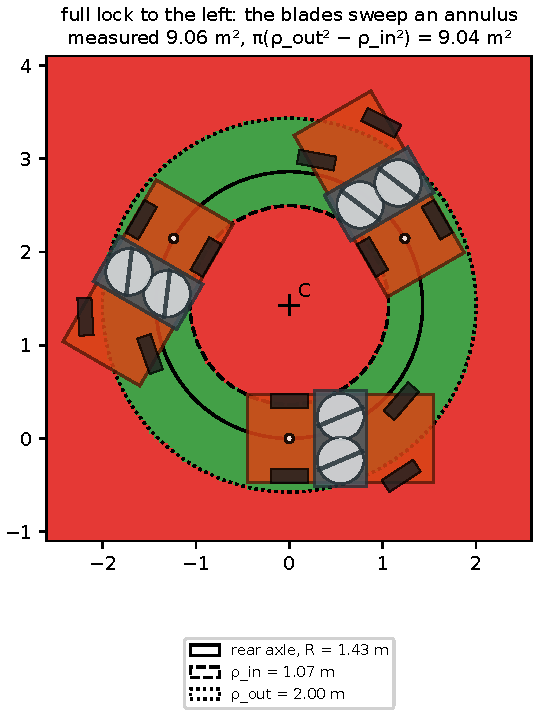
\includegraphics[width=0.52\textwidth]{figures/turning_circle}
  \caption{The mower driving a full circle at full lock to the left, drawn at
    three positions, and the area its blades cut, measured by the simulator
    (green: cut, red: not cut). $C$ is the centre of rotation. The rear axle
    $P$ follows the solid circle of radius $R = \SI{1.43}{\metre}$; the cut
    area is the annulus between $\rho_{\mathrm{in}} = \SI{1.07}{\metre}$
    (dashed) and $\rho_{\mathrm{out}} = \SI{2.00}{\metre}$ (dotted), larger
    than $R$ on the outside because the deck is ahead of the rear axle.}
  \label{fig:turningcircle}
\end{figure}

How much grass is cut per metre driven? Straight ahead, the blades cut a band
of width $w$, so $w$ square metres per metre. In a turn the answer changes.

\begin{proposition}{Area swept per metre}{weff}
  On an arc of curvature $\kappa \neq 0$ ($R = 1/|\kappa|$), the blades sweep
  new area at the rate of at most
  \[
    \weff(\kappa) \;=\; \frac{\rho_{\mathrm{out}}^2
      - \rho_{\mathrm{in}}^2}{2R}
  \]
  square metres per metre travelled by $P$, with equality when the blade
  annuli overlap (Proposition~\ref{prop:blades}). Straight ahead,
  $\weff(0) = w$.
\end{proposition}

\begin{proof}
  While the heading turns by $d\theta$, $P$ travels $ds = R\,d\theta$, and
  every point cut during that time lies in the sector of the annulus of
  angle $d\theta$, of area $\tfrac12(\rho_{\mathrm{out}}^2 -
  \rho_{\mathrm{in}}^2)\,d\theta$. Dividing by $ds = R\,d\theta$ gives the
  bound. When the annuli overlap, the swept region is the whole sector, so
  the bound is reached. Straight ahead, during $ds$ the blades sweep a
  rectangle $w \times ds$.
\end{proof}

\begin{example}{Effective width at full lock}{weffnum}
  With the radii of Example~\ref{ex:uncut}:
  \[
    \weff(\kmax) = \frac{2.0036^2 - 1.0656^2}{2 \times 1.4301}
    = \frac{4.0144 - 1.1355}{2.8602} = \SI{1.0065}{\metre},
  \]
  which is more than the cutting width $w = \SI{0.97}{\metre}$
  (Figure~\ref{fig:weff}).
\end{example}

\begin{figure}[ht]
  \centering
  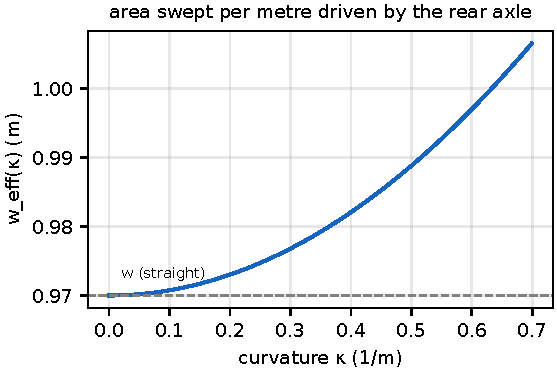
\includegraphics[width=0.55\textwidth]{figures/effective_width}
  \caption{Area swept by the blades per metre driven by the middle of the
    rear axle, as a function of the curvature, for the default mower. It
    grows from $w = \SI{0.97}{\metre}$ (straight) to \SI{1.0065}{\metre} at
    full lock ($\kmax = \SI{0.699}{\per\metre}$): in a turn, the deck is
    ahead of the rear axle and on the outside of its path, so it moves faster
    than $P$.}
  \label{fig:weff}
\end{figure}

\begin{inwords}
  In a turn, the blades on the outside travel farther than the rear axle,
  and those on the inside less; the outside wins, because area grows with
  the square of the radius. So a metre of turning cuts slightly more grass
  than a metre in a straight line. This is used in Chapter~\ref{ch:measuring}
  to bound how short a complete mowing path can be.
\end{inwords}

\begin{incode}
  \code{mowersim/mower.py}: \code{Mower} holds the dimensions
  (\code{min\_radius}, \code{max\_curvature}, \code{cutting\_width},
  \code{ackermann\_angles}). \code{mowersim/kinematics.py}: \code{advance}
  is Proposition~\ref{prop:arc}. \code{mowersim/coverage.py}:
  \code{effective\_width} is Proposition~\ref{prop:weff}. \code{python -m
  mowersim mower} draws the mower straight and at full lock.
\end{incode}
